\chapter{Two-Dimensional Radiative Transfer}
\begin{pycode}[2DRT]
name = '2DRT'
ch2DRT = texfigure.Manager(
    pytex,
    './03TwoDRT',
    number=3,
    python_dir='./03TwoDRT/python',
    fig_dir=   './03TwoDRT/Figs',
    data_dir=  './03TwoDRT/Data'
)
\end{pycode}

% \begin{itemize}
%     \item Adding a dimension to RT, formal solver etc.
%     \item Simulation setup.
%     \item Analysis.
%     \item Suggestions on visibility of this chromospheric glow with DKIST.
% \end{itemize}

It is clear that the world around us is multi-dimensional, but until this point, we have only considered radiative transfer in one-dimensional atmospheres.

All of the theory of radiative transfer discussed in previous chapters remains valid when applied to higher dimensional systems, with the exception of the description of the formal solver.
This is due to the non-local terms that appear within the MALI description (with diagonal $\Lambda$ operator) being handled by formal solver, which is responsible for computing the radiation field throughout the plasma from the local parameters and boundary conditions and thus coupling the atmospheric nodes to each other.
Once the radiation field has been computed it is then used as a local parameter in the rest of the iteration.
In fact, if the storage for the atmosphere is ``flattened'' into a one-dimensional form, the code from the plane-parallel case can (and should) be used to implement the iteration scheme.

In this chapter we shall first describe the extension of the \Lw{} framework to two dimensions (with the possibility of further extension), and then describe its application to the simulation of a flaring atmosphere illuminating an adjacent slab of quiet sun, along with potential implications for future observations at high resolution.

\section{The Formal Solver in Two-Dimensions}

Similarly to the plane-parallel formal solver used in \Lw{}, described in the previous chapter, we use the short-characteristics method to compute the radiation field throughout the atmosphere.
This approach was first employed in two-dimensions by \citet{Auer1994} using a limited parabolic scheme to avoid overshoot.
We assume the following basis: the $z$-axis is oriented as in the plane-parallel case, oriented vertically from photosphere to corona, the $x$-axis is perpendicular and co-planar to the $z$-axis (in the plane of the page for the following diagrams), and by the right-hand rule the $y$-axis is oriented into the plane of the page.
In the two-dimensional case it is assumed that the atmospheric parameters are homogenous along the $y$-axis, but vary along the $x$- and $z$-axes.
We assume that the atmosphere has a fixed stratification in $x$ and $z$, and that the atmospheric parameters are known at each intersection of these grids.

The mean intensity at each point will be computed similarly to the plane-parallel case; by integration of the local intensity over a weighted angular quadrature.
The Gauss-Legendre nodes used in the plane-parallel case are poorly suited to anisotropy that occurs in the two- and three-dimensional cases, and so we therefore employ the optimised quadratures of \citet{Stepan2020} in \Lw{}.

\begin{figure}
\centering
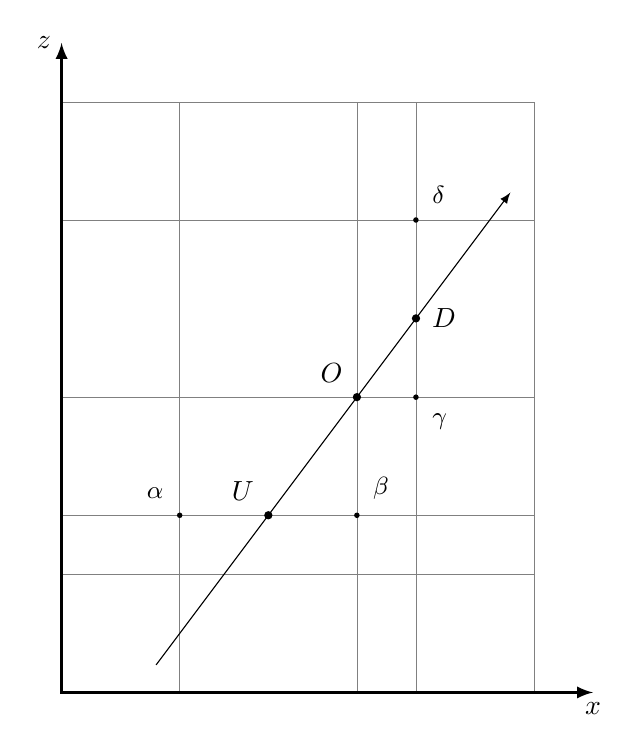
\begin{tikzpicture}[scale=1.5, line width=1pt, >=latex]
    \def\xcoords{1,2,3.5,4,5}
    \def\xmax{5}
    \def\ycoords{1,2,2.5,3.5,5,6}
    \def\ymax{6}
    \def\raym{4/3}
    \def\rayc{-7/6}

    \draw [help lines]
    \foreach \y in \ycoords {
        (1, \y) -- (\xmax, \y)
    }
    \foreach \x in \xcoords {
        (\x, 1) -- (\x, \ymax)
    };
    \draw [<->] ({\xmax+0.5}, 1) node[below] {$x$} -- (1,1) -- (1, {\ymax+0.5}) node[left] {$z$};
    \coordinate (O) at (3.5, 3.5);
    \node[circle, fill=black, inner sep=0 pt, minimum size=3pt, label=above left:{$O$}] at (O) {};
    \draw[->, domain=1.8:4.8, samples=10, thin] plot(\x, {\raym * (\x) + \rayc});
    \coordinate (D) at (4, {\raym * 4 + \rayc});
    \node[circle, fill=black, inner sep=0 pt, minimum size=3pt, label=right:{$D$}] at (D) {};
    \coordinate (U) at ({(2.5 - \rayc) / (\raym)}, 2.5);
    \node[circle, fill=black, inner sep=0 pt, minimum size=3pt, label=above left:{$U$}] at (U) {};

    \node[circle, fill=black, inner sep=0 pt, minimum size=2pt, label={[label distance=0.5mm]above left:{\small $\alpha$}}] at (2, 2.5) {};
    \node[circle, fill=black, inner sep=0 pt, minimum size=2pt, label={[label distance=0.5mm]above right:{\small $\beta$}}] at (3.5, 2.5) {};
    \node[circle, fill=black, inner sep=0 pt, minimum size=2pt, label={[label distance=0.5mm]below right:{\small $\gamma$}}] at (4, 3.5) {};
    \node[circle, fill=black, inner sep=0 pt, minimum size=2pt, label={[label distance=0.5mm]above right:{\small $\delta$}}] at (4, 5) {};
\end{tikzpicture}
\caption{Diagram of short characteristics scheme in two-dimensions.}
\label{Fig:Sc2d}
\end{figure}

For each ray prescribed by the angular quadrature the formal solver must perform one sweep through the grid.
The general case, that of an inclined ray ray travelling through the atmosphere is shown in, Fig.~\ref{Fig:Sc2d}.
In the case of this ray the formal solver must sweep first along $x$ and then along $z$, and the difficulties which can arise from this will be discussed in Sec.~\ref{Sec:2dEvalOrder}.
The points $U$ and $D$ refer to them being ``upwind'' and ``downwind'' of the point $O$ for which we are currently computing the intensity.
This can be explained by looking at the intersections of ray with the grid.
To compute the intensity in the direction of this ray at point $O$ using the short characteristics formulation we have, as in one-dimension,
\begin{equation}\label{Eq:MiniScDefinition}
   I_O = I_U e^{-(\tau_U - \tau_O)} + \int_{\tau_O}^{\tau_U} S(t) e^{-(t - \tau_O)}\, dt,
\end{equation}
where these terms have their usual meanings, $I_O$ is the intensity in this direction at $O$, $I_U$ is the intensity in this direction at $U$ and we have dropped the angular and frequency dependencies for clarity.
Thus, to compute the intensity at $O$, the intensity at $U$ must first be known.
As $U$ does not typically lie on a point of our discrete two-dimensional grid, the value of $I_U$ (and other quantities) are not computed directly by the formal solver, and must instead be interpolated from the values of grid points along the line $\alpha\beta$.

Following the short characteristic method, a functional form must be assigned to the variation of $S$ over the the line segment $[UO]$.
In the simplest case, this can again be a linear functional form, but due to the additional dimension for inhomogeneities in the two-dimensional case, unless the grid is very fine or the atmosphere very slowly varying, this may be a poor choice.
A higher order parametrisation of $S$ is likely to require the values of the source function at both $U$ and $D$, and possibly other points along this path.
Similarly to the cubic Bézier spline method used as standard in our plane-parallel code, we once again turn to monotonic Bézier splines for safe, smooth interpolation, minimising the presence of under and over-shoots.
The cubic method we apply in plane-parallel atmospheres requires four points along $UD$, which becomes less practical in higher dimensions, due to the large computational demands of the method.
Instead we choose the quadratic Bézier spline method, BESSER, of \citet{Stepan2013}, which will be briefly summarised here for the scalar case of the RTE.

\subsection{The BESSER method}

The BESSER method differs from other quadratic Bézier spline methods by ensuring the continuity of the first derivative of the interpolant at $O$.
Due to the large differences in optical depth between adjacent regions (e.g. $\tau_{UO}$ and $\tau_{OD}$) that are likely to occur in multi-dimensional cases with irregular grids, this method is designed so as to guarantee that if the values over $[UOD]$ are monotonic then the spline interpolant will remain monotonic.

The spline interpolant over the $[UO]$ interval is described by
\begin{equation}
    f(u) = (1-u)^2f_U + 2u(1-u)c_U + u^2f_O,\hspace{3em}u\in[0,1],
\end{equation}

where $f$ is the value of the parameter to be interpolated, $c_U$ is the functional value of the spline's control point, and $u$ is the normalised coordinate for the distance along $[UO]$.
The control points are points half way along an interval, defining the tangent to the spline at each end of the range i.e. $c_U O$ defines the tangent to the spline at $O$ and $U c_U$ defines the tangent to the spline at $U$.
If we denote the coordinates of our points along the ray $s_U$, $s_O$, and $s_D$ then we have $u = (s - s_U) / h_U$, where $h_U = s_U - s_O$.
An equivalent interpolation can be defined over the $[OD]$ segment.
The monotonicity (for monotonic $f_U$, $f_O$, $f_D$) and continuous first derivative of the interpolating functions at $O$ is ensured by
\begin{enumerate}
    \item Verify the monotonicity of $f_U$, $f_O$, $f_D$, and if $f_O$ is a local extremum then the control points $c_U$ and $c_D$ are set to $f_O$, giving a derivative of zero at $O$. As this is is the only possible solution for this case, the process stops here.

    \item Compute an estimate of the derivative at $O$, by using the derivative of the standard parabolic interpolation of $UOD$.

    \item Use this derivative to compute the initial values at the control points, by direct projection of the first derivative to their coordinates (as this defines a tangent to function at $O$).

    \item Check $c_U \in [f_U, f_O]$. If not, set $c_U$ to $f_U$ to correct for any new extremum and halt the process, as $c_D$ is not needed for the integration of the source function.

    \item Check $c_D \in [f_O, f_D]$. If not, set $c_D$ to $f_D$, and use this to compute a new value for the derivative at $O$, and follow the projection of this tangent to determine $c_U$ (due to the enforced continuity of the derivative at $O$).
\end{enumerate}
This process is described in more detail in \citet{Stepan2013}, but this covers the most important elements of the process.

\TODO{Do we modify to use the full value for $\tau_{OD}$?}
\TODO{Is this the correct what of expressing the difference between the control point, and the \emph{value} of the control point?}

Similarly to the plane-parallel case, we will solve the RTE in optical depth, due to its increased stability.
This interpolation method can be used to compute $\tau_{UO}$ and $\tau_{OD}$ by
\begin{align}
    \tau_{UO} &= \frac{1}{3}(\chi_U + \chi_O + \chi_{c_U}) (s_O - s_U),\\
    \tau_{OD} &= \frac{1}{2}(\chi_O + \chi_D) (s_D - s_O).
\end{align}
Note that a linear approximation was used for $\tau_{OD}$, as the previous process does not guarantee the calculation of $c_D$.
This could be modified to also use the quadratic spline method, which may be more robust, however the value of $\tau_{OD}$ rarely affects the final solution dramatically.

This method can now be applied to the source function but parametrised along $\tau$ rather that $s$.
The BESSER quadratic spline method is then used to compute the value of the source function control point $S_{c_U}$.
The integral in \eqref{Eq:MiniScDefinition} can now be evaluated, by using the prescribed quadratic spline variation of $S$ over the interval $[\tau_{U}, \tau_{O}]$.
Working through the maths we arrive at
\begin{equation}
    I_D = I_Ue^{-\tau_{UO}} + \omega_U S_U + \omega_O S_O + \omega_{c_U} S_{c_U},
\end{equation}
where,
{
\def\edt{e^{-\tau_{UO}}}
\def\tsq{\tau_{UO}^2}
\begin{align}
    \omega_U &= \frac{2 - (\tsq + 2\tau_{UO} + 2)\edt}{\tsq},\\
    \omega_O &= 2\frac{\tau_{UO} - 2 + \edt (\tau_{UO} + 2)}{\tsq},\\
    \omega_{c_U} &= 1 - 2 \frac{\edt + \tau_{UO} - 1}{\tsq}.
\end{align}
}

For small values of $\tau_{UO}$ the numerical precision of the exponential function becomes unreliable (in floating point arithmetic), so for this reason these are replaced with Taylor expansions for $\tau_{UO}\lesssim 0.1$.

An expression for the $\Lambda^*$ operator can then be devised equivalently to the process used previously for the plane-parallel case.
The source function is locally set to unity, and zero elsewhere.
This implies that $c_U$ is also set to 1.
Thus the local contribution to the radiation field is given by
\begin{equation}
    \Lambda^*(\nu, \vec{d}) = \omega_{c_U} + \omega_O,
\end{equation}
and remains related to $\Psi^*$ by the local opacity.

The equivalent integration and $\Lambda$ operator coefficients for a linear short characteristics approach can be computed similarly and are analagous to those computed in the one-dimensional case.

\subsection{Evaluation Order and Boundary Conditions}\label{Sec:2dEvalOrder}

Looking more closely at the order in which the formal solver needs to sweep the grid, we can see that the point $O$ for the ray discussed in the previous section (and shown in Fig.~\ref{Fig:Sc2d}) would be the 10th node to be solved, and this ordering is shown in Fig.~\ref{Fig:2DSweep}.
Most of the nodes on this figure are solved equivalently to this one, with all necessary quantities known at evaluation time provided the sweep order is preserved, but there are several question marks which require explanation.

\begin{figure}
\centering
\subimport{03TwoDRT/}{SweepOrder}
\caption{Diagram of sweep order in 2D}
\label{Fig:2DSweep}
\end{figure}

The {\color{TolBlue} blue} question marks along the $x$ axis all require values that must be computed from the boundary conditions.
The upper and lower boundary conditions in $z$ are typically taken to be described by a defined in-going radiation field (possibly zero or based on a black body).
The upper and lower boundaries in $x$ can be described by fixed boundary conditions, but it is also common to describe these with periodic boundary conditions where the ray wraps from one side of the grid to the other.
The {\color{TolTeal} teal} question marks along the upper $x$ boundary can then be interpreted in multiple ways; in the case of periodic boundary conditions they can be prolonged along the {\color{TolTeal} teal} arrows, and used in the same way as the previously described case.
If fixed boundary conditions are used then the intensity at these points must be computed by a linear formal solver indicated by the black arrows ending at the nodes labelled 4 and 8.

Finally, the region around the {\color{TolOrange} orange} question mark, the tail end of the arrow passing through node 11, requires some additional explanation.
In the configuration shown here, the arrow can stop at its intersection with the vertical line on which nodes 6 and 10 lie as the intensity information has been computed at both of these.
If an equivalent situation occurs at a periodic $x$ boundary, then a long characteristics approach will need to be applied to this ray.
This implies that the ray will need to be prolonged back to the previous intersection with a horizontal grid line, where the necessary intensity values can be interpolated, as is shown on this figure.
There are multiple options for treating the integration over the segment between this upwind point and the node.
Whilst it is possible to take this segment as a singular integration term, very inclined rays may cross multiple vertical grid lines and regions with dramatically varying parameters.
For this reason it is common to sub-step along this ray, performing an accumulated short-characteristics integration along each subinterval.

Another problem that may arise, closely related to choosing the correct upwind point, is that of velocity shifts in the medium.
\citet{VanNoort2002} discussed the possibility of the opacity over an integration integral being underestimated due to differing Doppler shifts at each end of the segment affecting the local opacity by a large margin (say from the core to the wing of the line).
As commented by \citet{Ibgui2013}, it is also possible for this effect to overestimate the opacity along this segment, in a similar manner.
The most common solution to this, proposed by \citet{VanNoort2002}, and explained in detail in \citet{Ibgui2013} is to subgrid along the ray.
The ray is then divided into subintervals along which the velocity may only change by a small (implementation defined) amount relative to the thermal velocity.
This approach can be very expensive when large Doppler shifts are present, due to the work involved in computing these segments, interpolating the necessary parameters to each start/end point (this will now require interpolation on both axes, rather than simply one as in the basic case discussed thus far), and the extra numerical integration steps.
This subgridding technique is not currently supported in \Lw{} but the code was designed with this method in mind, and a sensible location has been left for its implementation.

\subsection{Implementation Details}

The restrictive ordering of a formal solver sweep discussed in the previous section imposes constraints on the parallelisation of this algorithm.
% In the case of a single-threaded program, it is sufficient to obey this order, however, when distributing work across threads or multiple computing nodes it is essential that the necessary information be present to avoid computation stalls, or the use of uninitialsed data.
There is an in-depth discussion of an advanced spatial and frequency parallelisation algorithm for multi-dimensional radiative transfer in \citet{Stepan2013}, however in \Lw{} we assume that the entire simulation domain can be held in memory and the formal solver is parallelised in frequency, equivalently to the plane-parallel case.

The data structures for storing the atmospheric and population information in \Lw{} were updated to support two dimensional atmospheres, storing the data contiguously so as to be able to reuse the core iteration machinery from the plane-parallel case (as inspired by the RH code).
Two-dimensional formal solvers can be loaded from external libraries via the same interface as used for their one-dimensional counterparts, and through these interfaces we ensure the modularity of \Lw{}.
An equivalent interface is also defined for the interpolation function to be used in two-dimensions, giving flexibility in the interpolation order and any form of limiting used (which may need to be adapted to specific grids).
\Lw{} provides default implementations of the two-dimensional linear and BESSER short-characteristics formal solvers, along with linear and BESSER interpolation schemes for the necessary parameters.
The framework defaults to the BESSER formal solver with linear interpolation for the parameters.

For efficiency, the calculation of the ray-grid intersections is performed in a separate pre-pass to the formal solution, as this information can be reused for each formal solution using the same angular quadrature.
Whilst it is possible to compute the necessary parameter interpolation weights at this stage, we choose not to do this, as it would render the interpolation interface either more limited, or substantially more complex, due to the need to utilise different numbers of interpolation weights for different schemes.
We instead opt to store fractional indices which can be used in conjunction with the grid information in any interpolation procedure.
Using 64-bit arithmetic these are a concise and robust method for storing these locations.
By design, the intersection calculation is only performed for one upwind and downwind point
(excluding long characteristics that cross grid boundaries), as the second order method is considered to be a sufficient trade-off in terms of computational cost against accuracy.
This could easily be updated in the future, and we acknowledge that this is a limitation in terms of the two-dimensional formal solvers that can be loaded via the external interface.


\subsection{Validation}

\setpythontexautoprint{false}
\begin{pycode}[2DValidation]
# NOTE(cmo): Hack to minimise the number of times this session needs to be run
ch2DRT = texfigure.Manager(
    pytex,
    './03TwoDRT',
    number=3,
    python_dir='./03TwoDRT/python',
    fig_dir=   './03TwoDRT/Figs',
    data_dir=  './03TwoDRT/Data'
)

# def data_file_path(manager, fileName):
#     return os.path.join(manager.data_dir, fileName)

# twoDFilename = '2DPlotData.pickle'
# try:
#     with pickle.open(ch2DRT.data_file(twoDFilename), 'rb') as f:
#         data2d = pickle.load(f)
# except:
from lightweaver.fal import Falc82
from lightweaver.rh_atoms import H_6_atom, H_6_CRD_atom, H_3_atom, C_atom, O_atom, OI_ord_atom, Si_atom, Al_atom, CaII_atom, Fe_atom, FeI_atom, He_9_atom, He_atom, He_large_atom, MgII_atom, Mg_atom, N_atom, Na_atom, S_atom
import lightweaver as lw
import matplotlib.pyplot as plt
import time
import pickle
import numpy as np
from lightweaver.utils import NgOptions, get_default_molecule_path
from lightweaver.LwCompiled import FastBackground

atmos1d = Falc82()
atmos1d.quadrature(5)
x = (np.arange(5) * 5_000).astype(np.float64)
Nx = x.shape[0]
z = np.copy(atmos1d.height)
Nz = z.shape[0]
temperature = np.zeros((Nz, Nx))
temperature[...] = atmos1d.temperature[:, None]
vx = np.zeros((Nz, Nx))
vz = np.zeros((Nz, Nx))
vturb = np.zeros((Nz, Nx))
vturb[...] = atmos1d.vturb[:, None]
ne = np.zeros((Nz, Nx))
ne[...] = atmos1d.ne[:, None]
nHTot = np.zeros((Nz, Nx))
nHTot[...] = atmos1d.nHTot[:, None]
atmos = lw.Atmosphere.make_2d(height=z, x=x, temperature=temperature, vx=vx, vz=vz, vturb=vturb, ne=ne, nHTot=nHTot)
atmos.quadrature(6)

wave = np.linspace(853.9444, 854.9444, 501)
rayDir = 0.9

aSet = lw.RadiativeSet([H_6_atom(), C_atom(), O_atom(), Si_atom(), Al_atom(), CaII_atom(), Fe_atom(), He_atom(), Mg_atom(), N_atom(), Na_atom(), S_atom()])
aSet.set_active('Ca')
spect = aSet.compute_wavelength_grid()

eqPops1d = aSet.compute_eq_pops(atmos1d)
ctx1d = lw.Context(atmos1d, spect, eqPops1d, Nthreads=16, conserveCharge=False)

# dPopsStop = [1e-1, 1e-2, 1e-3, 1e-4]
dPopsStop = np.logspace(-1, -4, 10)
Iwave1ds = []
Iwaves = []

start1d = time.time()
for i in range(2):
    ctx1d.formal_sol_gamma_matrices()
dPops = [1.0]
currentStop = 0
for i in range(2000):
    ctx1d.formal_sol_gamma_matrices(lambdaIterate=False)
    dPops.append(ctx1d.stat_equil())
    if dPops[-1] < dPopsStop[currentStop]:
        Iwave1d = ctx1d.compute_rays(wave, rayDir)
        Iwave1ds.append(Iwave1d)
        currentStop += 1
    if dPops[-1] < 1e-4:
        print(i)
        break
end1d = time.time()
time1d = end1d - start1d
Niter1d = i

eqPops = aSet.compute_eq_pops(atmos)
start = time.time()
bgProvider = lambda *args: FastBackground(*args, Nthreads=16)
ctx = lw.Context(atmos, spect, eqPops, Nthreads=16, conserveCharge=False, backgroundProvider=bgProvider)

start = time.time()
for i in range(2):
    ctx.formal_sol_gamma_matrices()
dPops = [1.0]
currentStop = 0
for i in range(2000):
    ctx.formal_sol_gamma_matrices(lambdaIterate=False)
    dPops.append(ctx.stat_equil())
    if dPops[-1] < dPopsStop[currentStop]:
        Iwave = ctx.compute_rays(wave, rayDir)
        Iwaves.append(Iwave)
        currentStop += 1
    if dPops[-1] < 1e-4:
        print(i)
        break
end = time.time()
time2d = end - start
Niter2d = i

wave = np.linspace(853.9444, 854.9444, 501)
wave -= CaII_atom().lines[-1].lambda0
\end{pycode}
\setpythontexautoprint{true}

\begin{pycode}[2DValidation]
fig, ax = plt.subplots(2, 1, figsize=texfigure.figsize(pytex, scale=1, height_ratio=0.8))
ax[0].plot(wave, Iwave1d, label=r'1D Reference')
ax[0].set_xlim(wave[0], wave[-1])
for j in range(ctx.spect.I.shape[-1]):
    ax[0].plot(wave, Iwave[:, j], '--', label=('2D, $x={:.0f}$\,\si{{\kilo\metre}}'.format(atmos.x[j] / 1e3)))
ax[0].legend()
ax[0].set_ylabel(r'Specific Intensity [SI]')

ax[1].plot(wave, (Iwave[:, 2] - Iwave1d) / Iwave[:, 2])
ax[1].set_xlabel(r'$\Delta\lambda$ [\si{\nano\metre}]')
ax[1].set_ylabel(r'Relative Error')
lFig = ch2DRT.save_figure('2DValidation', fig, fext='.pgf')
lFig.caption = r'Validation of 2D formal solver.'
\end{pycode}

\begin{pycode}[2DValidation]
fig = plt.figure(figsize=texfigure.figsize(pytex, scale=1, height_ratio=0.7))
ax = plt.gca()

maxChanges = []
l2s = []

def l2_norm(x, y):
    return np.mean((x - y)**2)

for i in range(len(Iwaves)):
    maxChanges.append(np.max(np.abs(Iwaves[i][:, 2] - Iwave1ds[i])))
    l2s.append(l2_norm(Iwaves[i][:, 2], Iwave1ds[i]))

ax.plot(dPopsStop, maxChanges, '+-', label='Max Difference')
ax.invert_xaxis()
ax1 = ax.twinx()
ax1.plot(dPopsStop, l2s, '+-', label='L2 Norm', c='C1')
# ax.legend()
ax.set_xscale('log')
ax.set_yscale('log')
ax1.set_yscale('log')
ax.set_xlabel(r'$\mathrm{max}(\Delta n / n)$')
ax.set_ylabel(r'Absolute Maximum Difference', c='C0')
ax1.set_ylabel(r'L2 Norm', c='C1')

lFig = ch2DRT.save_figure('2DErrChange', fig, fext='.pgf')
lFig.caption = r'Differences between the 1 and 2D Formal Solvers (including ALI iteration procedure).'
\end{pycode}

\py[2DValidation]|ch2DRT.get_figure('2DValidation')|
\py[2DValidation]|ch2DRT.get_figure('2DErrChange')|

It is necessary to validate both the two-dimensional formal solver and its integration into the \Lw{} framework.
Here, we present a basic validation case, a horizontally homogenous FALC atmosphere, using five points in $x$, spaced \SI{5}{\kilo\metre} apart.
The boundary conditions in $x$ are periodic, thermalised at the photosphere, and no incoming radiation at the top of the atmosphere.
The standard configuration of \Lw{} in two-dimensions is used, i.e. BESSER formal solver and linear interpolation.
In Fig.~\ref{Fig:2DValidation} we show the comparison of a \CaLine{} computed using this two-dimensional method against the same model atom and atmosphere in a plane-parallel configuration.
Both of these are iterated until the maximum relative change in the \Caii{} populations is less than $10^{-4}$.
The outgoing radiation shown in the upper panel of this figure was synthesised for rays in the $x-z$ plane at $\mu_z = 0.9$.
Visually, the dashed lines, showing the solution from different $x$ locations using the two-dimensional formal solver overlie each other perfectly, showing that the output is homogenous across the $x$ axis, as is to be expected from this horizontally homogenous atmosphere with periodic boundary conditions.
There is a slight visible offset between the solutions generated from the plane-parallel and two-dimensional simulations, and the relative difference between these is shown in the lower panel of this figure.
We see that the relative difference is greatest in the line core, peaking at around 1.5\%.
Overall, this is very good agreement considering the different underlying methods used in the formal solvers.

In Fig.~\ref{Fig:2DErrChange} we show how the difference between the plane-parallel and two-dimensional models changes as the maximum relative population change decreases (i.e. as we approach convergence).
Further iterations beyond a maximum relative population change of $10^{-3}$ do not substantially improve the agreement between the two methods.
Thus, the situation shown in Fig.~\ref{Fig:2DValidation} is sufficiently converged to compare the final solutions of the two methods.

We find that the two-dimensional formal solver performs well, both in terms of accuracy and computational performance. For the example presented here the plane-parallel solution takes \py[2DValidation]|(r'\SI{{{:.3f}}}{{\second}}'.format(time1d))| and the two-dimensional solution takes \py[2DValidation]|(r'\SI{{{:.3f}}}{{\second}}'.format(time2d))| after \py[2DValidation]|Niter1d| and \py[2DValidation]|Niter2d| iterations respectively (this timing includes configuring the additional contexts and the formal solutions used for the convergence analysis shown in Fig.~\ref{Fig:2DErrChange}).
Both of these simulations were run with 16 threads on \TODO{machine name}.

Similar validation tests have been run for fixed boundary conditions and Doppler shifted atmospheres, all of which yielded extremely satisfactory results.

\section{2D Simulation Configuration}

\begin{figure}
\centering
\subimport{03TwoDRT/}{SimConfig}
\caption{Sim Config}
\label{Fig:2DSimConfig}
\end{figure}

Flare models produce huge changes in the radiation field, in both lines and continua.
These flares are typically modelled in a plane-parallel context and we analyse the radiation leaving the top of this plane-parallel atmosphere.
In reality, the flaring kernels that we are simulating with these RHD models are likely small; on the scale of 10s to 100s of \si{\kilo\metre} \NeedRef{} and represent an estimate of the conditions in the core of a heated flux-tube.
As the resolution of solar telescopes increases, so does their ability to resolve spatial effects tangential to the solar surface (henceforth horizontal).
The lack of horizontal atmospheric homogeneity, that is not currently accounted for in these models, may produce complex intensity structures resolvable with these new telescopes as the huge outgoing flux of radiation from the flare core impinges and interacts with neighbouring plasma.

It is reasonable to suggest that the plasma neighbouring the flare is substantially cooler, both due to the lack of direct heating, and the low strength of cross-field conduction relative to that along the field, however the radiation is not affected by these limitations.
Thus, we will investigate the effects of illumination from a neighbouring plane-parallel flare model on a two-dimensional slab of plasma representing the chromosphere, with a time-dependent radiative treatment of both of these.
This model can then serve as an approximate investigation of the outgoing radiation from the slab, as well as the depth of radiation penetration, effects on the atomic populations, and observable signatures.

Our simulation is set up as shown in Fig.~\ref{Fig:2DSimConfig}; the primary simulation domain is a \SI{2}{\mega\metre} wide slab of plasma initially set to the quiet sun atmosphere used for the RADYN simulation.
On one side of this slab we place the RADYN simulation, and compute the intensity along each ray of the angular quadrature used for the 2D slab, at each depth in the simulation.
The other $x$ boundary is treated equivalently, but using the fixed initial quiet sun atmosphere from the RADYN simulation and the 2D slab.

Similarly to the process described in the previous chapter a time-dependent simulation is run, again reprocessing the theormdynamic atmospheric properties using RADYN's internal timestep.
The separate simulation components of this model share a $z$ stratification based on a combination of RADYN's grids used for both the initial quiet sun atmosphere and the current timestep.
This method ensures that 450 points are spaced across the atmosphere in $z$ and provide sufficient resolution for the transition region of both the quiet sun model \emph{and} that of the flare model.
The populations are interpolated between the $z$ grids from one step to the next, and locally scaled to follow the mass density (this is typically a small adjustment, but without it errors can grow as points move through the transition region).
The electron density in the RADYN atmosphere is model is loaded from the RADYN output, and charge is conserved in the 2D slab using the secondary Newton-Raphson iteration procedure discussed previously.
The 6 rays per octant of the unit sphere quadrature of \citet{Stepan2020} was chosen, as the plasma in the 2D slab is static and these rays capture more than enough detail to describe the radiation field leaving the plane parallel model (where the radiative transfer model natively uses 5 Gauss-Legendre rays per quadrant of the unit disc).
In addition to the 450 points in $z$, we use 41 linearly spaced points in $x$ to discretise the two-dimensional atmosphere.
As these 40 points span \SI{2}{\mega\metre} each point is spaced \SI{50}{\kilo\metre} apart.
Due to the very fine $z$ spacing that often occurs due to the strong gradients in the transition region, many of the 2D cells have an aspect ratio very far from square.
This does not appear to have affected the results, as a temporally shortened version of one of the simulations was run with the $x$ grid spacing halved, and no substantial change in outgoing intensity was found.

The left-most column of the 2D slab requires special treatment due to the nature of fixed boundary conditions in RT simulations that will be discussed here.
The incoming radiation from the flare model is specified for each ray and depth in the first column of the atmosphere.
As the intensity is specified for all incoming (rightgoing) rays here, it cannot be calculated taking into account the local parameters, meanwhile the outgoing (leftgoing) rays \emph{do} take into account the local parameters, and then inform the local operator acting on these populations.
Thus, if this column has its thermodynamic properties fixed to those of the initial quiet sun model, it behaves as if it is only receiving radiation from the right, and only being affected by the flare in a ``second-hand'' sense.
This leads to a dark first column in the two-dimensional synthesis.
To minimise these effects we copy the flare atmosphere into this first column, and hold the populations fixed over each timestep.
These populations are then consistent with the adjacent plane-parallel atmosphere and the radiation emerging from it which is used as a fixed boundary condition.
There should not be any need to perform the same process at the quiet sun boundary, as it is placed \SI{2}{\mega\metre} away and should change very little over the course of the simulation, remaining consistent on both sides of the boundary.

This configuration produces the outgoing intensity at 12 different angles from each of the 41 cells in $x$.
We can use the symmetric definition of these to produce the radiation observed by a theoretical slit spectrograph viewing the sun from a particular inclination with the flare in the centre of the slit.
This is shown in Fig.~\ref{Fig:2DSimFlipped}; for an observation inclined as shown we are observing the radiation along the blue arrows.
For the reflected atmosphere, the blue arrow shown is equivalent to the magenta arrow from the simulated atmosphere.

\begin{figure}
\centering
\subimport{03TwoDRT/}{SimFlipped}
\caption{Using the single simulation shown in Fig.~\ref{Fig:2DSimConfig} to investigate the radiation observed by a slit spectrograph looking across the flaring region. The radiation emitted along the blue arrow from the reflected atmosphere is the same as that from the magenta arrow in the simulated atmosphere.}
\label{Fig:2DSimFlipped}
\end{figure}

We will focus primarily on these inclined observations as flares are extremely unlikely to occur at disc centre and the effects of inclination are therefore important.
Even a slight inclination can have a large effect, and in the following we will focus primarily on the most vertical ray present in our quadrature, with an angle of \SI{18}{\degree} to the surface normal.
Only 1/25 of the visible solar disc has a viewing angle smaller than this, so inclination effects will be at least this significant for the majority of observed flares.

In this simulation we use the same model atoms as the previous chapter, with both hydrogen and calcium being set as active species.
This simulation is carried out for two different flare models illuminating the 2D slab; the same F9 and F10 models of Chapter~\ref{Chap:TimeDepRt} (including the Lyman line photoionisation effects!).
We will now showcase the results of these simulations, looking at both the observable effects and the population changes internal to the slab, focusing on the \Ha{} and \CaLine{} spectral lines, before comparing these to observations taken with the CRISP instrument on the SST.


\section{Simulation Results}

Due to the additional complexity of the two-dimensional simulation these models are substantially more computationally intensive to compute, both due to larger number of points to be solved as well as the increased angular samples and interpolations needed at each point.
The F9 simulation, consisting of 1793 internal timesteps takes $\sim$2,300 CPU hours, and the F10 model, with 5996 timesteps takes $\sim$10,000 CPU hours on the hercules machine \TODO{machines}.
{\color{Red} The code for these simulations is present in the MsLightweaver repository on the RefinedGrid2d branch.} \TODO{DOI - when sims have rerun}.

\subsection{Observed Radiation}


% Is there a way we can characterise the scattering? Destruction probability?

% Flipping viewing angle is the same as observing symmetric point E/W. Make viewing angle diagram and discuss.

\begin{pycode}[2DRT]
import zarr
import matplotlib.gridspec as gridspec


def plot_rel_change_2d(fig, d, wl, wlOffset, position, angularIdx, enhancementLine=0.4):
    fig.clf()

    xEdges = (np.arange(d['xAxis'].shape[0]+1) - 0.5) * d['xAxis'][1]
    xEdges /= 1e6
    spec = gridspec.GridSpec(nrows=3, ncols=2, width_ratios=[1.75,1], figure=fig)
    xAxis = d['xAxis'][...] / 1e6
    wavelength = d['wavelength']

    timeEdges = np.concatenate(([0],
                                0.5 * (d.time[1:] + d.time[:-1]),
                                [d.time[-1]]))

    Idata = d['I'][:, :, angularIdx, :][...]
    IChangeArr = (Idata - Idata[:, :, -1][:, :, None]) / Idata[:, :, -1][:, :, None]

    offset = wlOffset

    change1 = IChangeArr[:, wl-offset, :]
    line1 = np.zeros(IChangeArr.shape[0])
    for t in range(change1.shape[0]):
        for k in range(change1.shape[1]-1, -1, -1):
            if change1[t, k] > enhancementLine:
                line1[t] = xAxis[k]
                break
    change2 = IChangeArr[:, wl, :]
    line2 = np.zeros(IChangeArr.shape[0])
    for t in range(change1.shape[0]):
        for k in range(change1.shape[1]-1, -1, -1):
            if change2[t, k] > enhancementLine:
                line2[t] = xAxis[k]
                break
    change3 = IChangeArr[:, wl+offset, :]
    line3 = np.zeros(IChangeArr.shape[0])
    for t in range(change1.shape[0]):
        for k in range(change1.shape[1]-1, -1, -1):
            if change3[t, k] > enhancementLine:
                line3[t] = xAxis[k]
                break

    ax = fig.add_subplot(spec[0, 0])
    change = IChangeArr[:, wl-offset, :]
    mesh = ax.pcolormesh(timeEdges, xEdges, change1.T, cmap='Greys_r', rasterized=True)
    ax.plot(d['time'], line1)
    ax.set_title(r'$\lambda={:.4f}$ nm'.format(wavelength[wl-offset]), fontdict={'fontsize': 11})
    ax.tick_params(axis='x', labelbottom=False)
    ax.set_ylabel('Extent [Mm]', fontdict={'fontsize': 11})
    ax.set_ylim(None, 1.5)
    cax = fig.colorbar(mesh, ax=ax)
    cax.ax.tick_params(axis='y', direction='out')

    ax = fig.add_subplot(spec[1, 0])
    change = IChangeArr[:, wl, :]
    mesh = ax.pcolormesh(timeEdges, xEdges, change2.T, cmap='Greys_r', rasterized=True)
    ax.plot(d['time'], line2)
    ax.set_title(r'$\lambda={:.4f}$ nm'.format(wavelength[wl]), fontdict={'fontsize': 11})
    ax.tick_params(axis='x', labelbottom=False)
    ax.set_ylabel('Extent [Mm]', fontdict={'fontsize': 11})
    ax.set_ylim(None, 1.5)
    cax = fig.colorbar(mesh, ax=ax)
    cax.ax.tick_params(axis='y', direction='out')

    ax = fig.add_subplot(spec[2, 0])
    change = IChangeArr[:, wl+offset, :]
    mesh = ax.pcolormesh(timeEdges, xEdges, change3.T, cmap='Greys_r', rasterized=True)
    ax.plot(d['time'], line3)
    ax.set_title(r'$\lambda={:.4f}$ nm'.format(wavelength[wl+offset]), fontdict={'fontsize': 11})
    ax.set_xlabel('Time [s]')
    ax.set_ylabel('Extent [Mm]', fontdict={'fontsize': 11})
    ax.set_ylim(None, 1.5)
    cax = fig.colorbar(mesh, ax=ax)
    cax.ax.tick_params(axis='y', direction='out')

    ax = fig.add_subplot(spec[:, 1])
    lineTimes = np.array([0, 4, 8, 10, 12, 16, 20, 25, 30])
    timeIndices = np.array([np.where(d['time'][...] == t)[0].squeeze() for t in lineTimes])
    for timeIdx in timeIndices:
        ax.plot(wavelength - wavelength[wl], Idata[timeIdx, :, position], label='{:.0f} s'.format(d['time'][timeIdx]))
    localScale = wavelength[wl+1] - wavelength[wl]
    ax.set_xlim(-localScale*70, localScale*70)
    ax.axvline(wavelength[wl] - wavelength[wl])
    ax.axvline(wavelength[wl-offset] - wavelength[wl], c='C1', ls='--')
    ax.axvline(wavelength[wl+offset] - wavelength[wl], c='C1', ls='--')
    ax.legend(loc=(0.65, 0.01), frameon=False, handlelength=1.0, handletextpad=0.6, labelspacing=0.35)
    ax.set_xlabel('$\Delta\lambda$ [nm]')
    ax.set_ylabel('Specific Intensity [SI]')

#         fig.suptitle('F9 into RADYN')
#         fig.suptitle(r'Ca ɪɪ 8542 $\AA$ F9 Heating')
    # fig.suptitle(r'H$-\alpha$ F9 Heating Flare atmosphere')
    fig.tight_layout()

dataRad = zarr.convenience.open(ch2DRT.data_file('F9_flat_450_41_nr_1stColCopy_besser_qsbc_radiation_thesis.zip'))
fig = plt.figure(figsize=texfigure.figsize(pytex, scale=1, height_ratio=0.7))
angularIdx = 1
plot_rel_change_2d(fig, dataRad, 743, 15, 2, angularIdx)
fig.tight_layout()
lFig = ch2DRT.save_figure('2DHaF9', fig, fext='.pgf', dpi=500)
lFig.caption = r'\Ha{} for 2D F9 Case.'

\end{pycode}

% \py[2DRT]|ch2DRT.get_figure('2DHaF9')|

\begin{pycode}[2DRT]
fig = plt.figure(figsize=texfigure.figsize(pytex, scale=1, height_ratio=0.7))
angularIdx = 1
plot_rel_change_2d(fig, dataRad, 927, 7, 2, angularIdx)
fig.tight_layout()
lFig = ch2DRT.save_figure('2DCaF9', fig, fext='.pgf', dpi=500)
lFig.caption = r'\CaLine{} for 2D F9 Case.'
\end{pycode}

% \py[2DRT]|ch2DRT.get_figure('2DCaF9')|

\begin{pycode}[2DRT]
fig = plt.figure(figsize=texfigure.figsize(pytex, scale=1, height_ratio=0.7))

angularIdx = 3
plot_rel_change_2d(fig, dataRad, 743, 15, 2, angularIdx)
fig.tight_layout()
lFig = ch2DRT.save_figure('2DHaF9Away', fig, fext='.pgf', dpi=500)
lFig.caption = r'\Ha{} for 2D F9 Case. Away from ribbon.'
\end{pycode}

% \py[2DRT]|ch2DRT.get_figure('2DHaF9Away')|

\begin{pycode}[2DRT]
fig = plt.figure(figsize=texfigure.figsize(pytex, scale=1, height_ratio=0.7))
angularIdx = 3
plot_rel_change_2d(fig, dataRad, 927, 7, 2, angularIdx)
fig.tight_layout()
lFig = ch2DRT.save_figure('2DCaF9Away', fig, fext='.pgf', dpi=500)
lFig.caption = r'\CaLine{} for 2D F9 Case. Away from ribbon'
\end{pycode}

% \py[2DRT]|ch2DRT.get_figure('2DCaF9Away')|

\begin{pycode}[2DRT]
def plot_2d_rad(ax, dataRad, time, waveRange):
    wavelength = dataRad['wavelength']
    wavelengthEdges = np.concatenate(([wavelength[0]], 0.5 * (wavelength[1:] + wavelength[:-1]), [wavelength[-1]]))
    x = dataRad['xAxis'][...] / 1e6
    xEdges = np.concatenate(([x[0]], 0.5 * (x[1:] + x[:-1]), [x[-1]]))

    timeIdx = np.searchsorted(dataRad['time'][...], time)
    waveCentre = 0.5 * (waveRange[0] + waveRange[1])

    Itowards = dataRad['I'][timeIdx, :, 1, :]
    Iaway = dataRad['I'][timeIdx, :, 3, :]
    Imax = max(dataRad['I'][:, :, 1, :].max(), dataRad['I'][:, :, 3, :].max())
    Imin = min(dataRad['I'][:, :, 1, :].min(), dataRad['I'][:, :, 3, :].min())
    ax.pcolormesh(wavelengthEdges - waveCentre, xEdges, Itowards.T, vmin=Imin, vmax=Imax, cmap='Greys_r', rasterized=True)
    ax.pcolormesh(wavelengthEdges - waveCentre, -xEdges, Iaway.T, vmin=Imin, vmax=Imax, cmap='Greys_r', rasterized=True)
    ax.axhline(0, c='r', alpha=0.6)
    ax.set_xlim(waveRange[0] - waveCentre, waveRange[1] - waveCentre)

fig, ax = plt.subplots(2,2, figsize=texfigure.figsize(pytex, scale=1, height_ratio=0.7))
waveRangeHa = (656.376, 656.576)
plot_2d_rad(ax[0,0], dataRad, 5, waveRangeHa)
ax[0,0].set_ylabel('$x$ [Mm]')
ax[0,0].set_title('5 s')
ax[0,0].set_xticklabels([])
plot_2d_rad(ax[0,1], dataRad, 10, waveRangeHa)
ax[0,1].set_title('10 s')
ax[0,1].set_xticklabels([])
ax[0,1].set_yticklabels([])
plot_2d_rad(ax[1,0], dataRad, 15, waveRangeHa)
ax[1,0].set_title('15 s')
ax[1,0].set_ylabel('$x$ [Mm]')
ax[1,0].set_xlabel('$\Delta\lambda$ [nm]')
plot_2d_rad(ax[1,1], dataRad, 25, waveRangeHa)
ax[1,1].set_title('25 s')
ax[1,1].set_xlabel('$\Delta\lambda$ [nm]')
ax[1,1].set_yticklabels([])

lFig = ch2DRT.save_figure('HaFull2dPlot', fig, fext='.pgf', dpi=500)
lFig.caption = r"\Ha{} intensity on both sides of the ``flare'' at different points during the F9 simulation."

fig, ax = plt.subplots(2,2, figsize=texfigure.figsize(pytex, scale=1, height_ratio=0.7))
waveRangeCa = (854.3444, 854.5444)
plot_2d_rad(ax[0,0], dataRad, 5, waveRangeCa)
ax[0,0].set_ylabel('$x$ [Mm]')
ax[0,0].set_title('5 s')
ax[0,0].set_xticklabels([])
plot_2d_rad(ax[0,1], dataRad, 10, waveRangeCa)
ax[0,1].set_title('10 s')
ax[0,1].set_xticklabels([])
ax[0,1].set_yticklabels([])
plot_2d_rad(ax[1,0], dataRad, 15, waveRangeCa)
ax[1,0].set_title('15 s')
ax[1,0].set_ylabel('$x$ [Mm]')
ax[1,0].set_xlabel('$\Delta\lambda$ [nm]')
plot_2d_rad(ax[1,1], dataRad, 25, waveRangeCa)
ax[1,1].set_title('25 s')
ax[1,1].set_xlabel('$\Delta\lambda$ [nm]')
ax[1,1].set_yticklabels([])

lFig = ch2DRT.save_figure('CaFull2dPlot', fig, fext='.pgf', dpi=500)
lFig.caption = r"\CaLine{} intensity on both sides of the ``flare'' at different points during the F9 simulation."
\end{pycode}

\py[2DRT]|ch2DRT.get_figure('HaFull2dPlot')|

The emergent radiation from the F9 simulation is shown for \Ha{} and \CaLine{} in Figs.~\ref{Fig:HaFull2dPlot} and \ref{Fig:CaFull2dPlot} respectively.
These are presented as described in Fig.~\ref{Fig:2DSimFlipped} with the reflected side shown in negative $x$.
Here we assume that the flaring atmosphere has infinitesimal width and is shown with the horizontal red line.
The intensity scale is constant for all timesteps for each line.
Immediately in both of these figures we see a large asymmetry between the observation of each side of the flare.
This is likely due to the rays observed from positive $x$ both scattering light from the flare and directly intersecting the flaring atmosphere.
There is some enhancement in the negative $x$ region, presenting as a narrowing of the line core in \Ha{} and enhancement of the core of \CaLine{}, but it is much less significant than that present in the positive $x$ region.
Despite the horizontal uniformity of plasma properties in this atmosphere, there is substantial variation in the observed radiation.

We note that for both spectral lines the far wings and continuum remain constant throughout the simulation.
This will be discussed more later, when the effects on the populations are investigated.

\def\regiona{$0-\SI{0.5}{\mega\metre}$}

\py[2DRT]|ch2DRT.get_figure('CaFull2dPlot')|

Taking a more detailed look at the \Ha{} line profiles shown in Fig.~\ref{Fig:HaFull2dPlot}, during heating ($t=\SI{5}{\second}$) we see a widened line profile with enhanced ``horns'' in both the red and blue wings over $0-\SI{0.5}{\mega\metre}$, a filling-in of the line core over $0.5-\SI{1}{\mega\metre}$, and a smooth return to the quiet sun line profile over the remained of the simulation.
In the negative $x$ region we see that the line core is less deep near the flare, decaying back to pre-flare levels over the \SI{2}{\mega\metre} extent.
The situation is similar at the end of the heating ($t=\SI{10}{\second}$), but here the core is driven into emission in the $0-\SI{0.5}{\mega\metre}$ region and remains in absorption, although enhanced through the rest of this region as it smoothly transitions back to its quiet sun shape.
A slight asymmetry of the red wing starts to appear here in the $0-\SI{0.5}{\mega\metre}$ region.
The negative $x$ region remains similar to $t=\SI{5}{\second}$ although the line core is less enhanced immediately adjacent to the flare.
Some time after the heating has ended ($t=\SI{15}{\second}$ and $t=\SI{25}{\second}$), the brightening in the blue wing over the \regiona{} region is now a dimming, but there remains an enhancement in the red wing.
The remainder of these timesteps remain similer to the $t=\SI{10}{\second}$ line profile, presenting an enhanced core (remaining in absorption) that slowly returns to its quiet sun form as distance from the flare illumination increases.

The \CaLine{} line profiles in the F9 simulation shown in Fig.~\ref{Fig:CaFull2dPlot} tell a similar story to the \Ha{} line profiles, although the line width does not vary noticeably throughout the simulation.
The line is strongly enhanced in emission over the \regiona{} region for $t=\SI{5}{\second}$ and $t=\SI{10}{\second}$, with a slight red asymmetry.
At later times this line remains in emission with a significant red asymmetry.
Throughout the simulation the line smoothly transitions back from its enhanced shape to its quiet sun profile at the $x=\SI{2}{\mega\metre}$ boundary.
The negative $x$ region presents slight core enhancement, stronger during heating, before decaying slowly after heating.

\TODO{F10 results.}
\TODO{Where do the ``wings'' start?}

We see that these optical line profiles can present significant core enhancements up to almost \SI{1}{\mega\metre} away from the flare boundary in these simulations when looking at a viewing angle that intersects this boundary (i.e. the positive $x$ region).
There are only modest changes for viewing angles where this is not the case (the negative $x$ region).
In both cases the line wings do not change significantly and we shall investigate this further by looking at how the level populations are affected by this incident radiation.

\subsubsection{Importance of time-dependence}

Due to the need to solve the radiative transfer problem at every timestep in the \Radyn{} simulation, the full time-dependent treatment is extremely computationally intensive.
If these effects are not important then the style of simulation presented here can be accelerated dramatically by performing a statistical equilibrium solution for the slab illuminated by the flaring boundary at each timestep of interest (which is likely to be many fewer than the total number of timesteps needed for the time-dependent solution).

\begin{pycode}[2DRT]
# NOTE(cmo): This is just the direct MsLw2d.zarr that came out of our
# simulation doing 0 and then jumping to 10s. Needs special handling, compared
# to other preprocessed ones.
statEq2d = zarr.convenience.open(ch2DRT.data_file('F9_flat_450_41_StatEqUpdated_t10_1stColCopy_besser_MsLw2d_thesis.zip'))

def plot_stat_eq_comparison(fig, dataRadTd, dataRad, waveRange):
    wavelength = dataRad['SimParams/wavelength']
    wavelengthEdges = np.concatenate(([wavelength[0]], 0.5 * (wavelength[1:] + wavelength[:-1]), [wavelength[-1]]))
    x = dataRad['SimParams/xAxis'][...] / 1e6
    xEdges = np.concatenate(([x[0]], 0.5 * (x[1:] + x[:-1]), [x[-1]]))

    xTd = dataRadTd['xAxis'][...] / 1e6
    xEdgesTd = np.concatenate(([xTd[0]], 0.5 * (xTd[1:] + xTd[:-1]), [xTd[-1]]))

    timeIdx = 1
    timeTd = 10.0
    timeIdxTd = np.searchsorted(dataRadTd['time'][...], timeTd)

    Itowards = dataRad['SimOutput/Radiation/I'][timeIdx, :, 5, :]
    ItowardsTd = dataRadTd['I'][timeIdxTd, :, 1, :]
    Iaway = dataRad['SimOutput/Radiation/I'][timeIdx, :, 11, :]
    IawayTd = dataRadTd['I'][timeIdxTd, :, 3, :]

    minWlIdx = np.searchsorted(wavelength, waveRange[0]) - 1
    maxWlIdx = np.searchsorted(wavelength, waveRange[1]) + 1
    Imax = max(Itowards[minWlIdx:maxWlIdx].max(), Iaway[minWlIdx:maxWlIdx].max())
    Imin = min(Itowards[minWlIdx:maxWlIdx].min(), Iaway[minWlIdx:maxWlIdx].min())
    spec = gridspec.GridSpec(nrows=1, ncols=2)
    ax = fig.add_subplot(spec[0])

    ax.pcolormesh(wavelengthEdges, xEdges, Itowards.T, vmin=Imin, vmax=Imax, cmap='Greys_r', rasterized=True)
    ax.pcolormesh(wavelengthEdges, -xEdges, Iaway.T, vmin=Imin, vmax=Imax, cmap='Greys_r', rasterized=True)
    ax.axhline(0, c='r', alpha=0.6)
    ax.set_xlim(*waveRange)
    ax.set_title('Statistical Equilibrium')
    ax.set_xlabel('$\lambda$ [nm]')
    ax.set_ylabel('$x$ [Mm]')

    ax = fig.add_subplot(spec[1])
    ax.pcolormesh(wavelengthEdges, xEdgesTd, ItowardsTd.T, vmin=Imin, vmax=Imax, cmap='Greys_r', rasterized=True)
    ax.pcolormesh(wavelengthEdges, -xEdgesTd, IawayTd.T, vmin=Imin, vmax=Imax, cmap='Greys_r', rasterized=True)
    ax.axhline(0, c='r', alpha=0.6)
    ax.set_xlim(*waveRange)
    ax.set_title('Time-Dependent')
    ax.set_xlabel('$\lambda$ [nm]')
    ax.set_yticklabels([])

fig = plt.figure(figsize=texfigure.figsize(pytex, scale=1, height_ratio=0.55))
plot_stat_eq_comparison(fig, dataRad, statEq2d, (656.376, 656.576))

lFig = ch2DRT.save_figure('2dCompareStatEqTimeDep', fig, fext='.pgf', dpi=500)
lFig.caption = r'Comparison of statistical equilibrium and time-dependent treatments at $t=\SI{10}{\second}$ for two-dimensional slab case.'

from scipy.integrate import trapezoid
import astropy.units as u
def plot_integrated_line_intensity(fig, dataRadTd, dataRad, centralWavelength, halfWidth):
    wavelength = dataRad['SimParams/wavelength']
    wavelengthEdges = np.concatenate(([wavelength[0]], 0.5 * (wavelength[1:] + wavelength[:-1]), [wavelength[-1]]))
    x = dataRad['SimParams/xAxis'][...] / 1e6
    xEdges = np.concatenate(([x[0]], 0.5 * (x[1:] + x[:-1]), [x[-1]]))

    xTd = dataRadTd['xAxis'][...] / 1e6
    xEdgesTd = np.concatenate(([xTd[0]], 0.5 * (xTd[1:] + xTd[:-1]), [xTd[-1]]))

    timeIdx = 1
    timeTd = 10.0
    timeIdxTd = np.searchsorted(dataRadTd['time'][...], timeTd)

    Itowards = dataRad['SimOutput/Radiation/I'][timeIdx, :, 5, :]
    ItowardsTd = dataRadTd['I'][timeIdxTd, :, 1, :]
    Iaway = dataRad['SimOutput/Radiation/I'][timeIdx, :, 11, :]
    IawayTd = dataRadTd['I'][timeIdxTd, :, 3, :]

    waveRange = (centralWavelength - halfWidth, centralWavelength + halfWidth)
    minWlIdx = np.searchsorted(wavelength, waveRange[0]) - 1
    maxWlIdx = np.searchsorted(wavelength, waveRange[1]) + 1

    intItowards = []
    for xi in range(Itowards.shape[1]):
        intItowards.append(-trapezoid(Itowards[minWlIdx:maxWlIdx, xi],
                           (wavelength[minWlIdx:maxWlIdx] << u.nm).to(u.Hz,
                                      equivalencies=u.spectral())).value)
    intIaway = []
    for xi in range(Iaway.shape[1]):
        intIaway.append(-trapezoid(Iaway[minWlIdx:maxWlIdx, xi],
                        (wavelength[minWlIdx:maxWlIdx] << u.nm).to(u.Hz,
                                   equivalencies=u.spectral())).value)
    intItowardsTd = []
    for xi in range(ItowardsTd.shape[1]):
        intItowardsTd.append(-trapezoid(ItowardsTd[minWlIdx:maxWlIdx, xi],
                             (wavelength[minWlIdx:maxWlIdx] << u.nm).to(u.Hz,
                                        equivalencies=u.spectral())).value)
    intIawayTd = []
    for xi in range(IawayTd.shape[1]):
        intIawayTd.append(-trapezoid(IawayTd[minWlIdx:maxWlIdx, xi],
                          (wavelength[minWlIdx:maxWlIdx] << u.nm).to(u.Hz,
                                     equivalencies=u.spectral())).value)

    ax = fig.gca()
    ax.plot(x, intItowards, c='C0', label='Statistical Equilibrium')
    ax.plot(-x, intIaway, c='C0')
    ax.plot(x, intItowardsTd, c='C1', label='Time-Dependent')
    ax.plot(-x, intIawayTd, c='C1')
    ax.set_ylabel(r'Intensity [\si{\joule\per\second\per\square\metre\per\steradian}]')
    ax.set_xlabel('$x$ [Mm]')
    ax.legend(frameon=False)


fig = plt.figure(figsize=texfigure.figsize(pytex, scale=1, height_ratio=0.55))
plot_integrated_line_intensity(fig, dataRad, statEq2d, 656.476, 0.2)
lFig = ch2DRT.save_figure('2dCompareIntegratedHa', fig, fext='.pgf')
lFig.caption = r'Integrated intensity of H$\alpha$ lines shown in Fig.~\ref{Fig:2dCompareStatEqTimeDep} as a function of $x$ position.'

fig = plt.figure(figsize=texfigure.figsize(pytex, scale=1, height_ratio=0.55))
plot_integrated_line_intensity(fig, dataRad, statEq2d, 854.4444, 0.1)
lFig = ch2DRT.save_figure('2dCompareIntegratedCa', fig, fext='.pgf')
lFig.caption = r'Integrated intensity of Ca\,\textsc{ii}\,\SI{854.2}{\nano\metre} lines treated with time dependence and statistical equilibrium as a function of $x$ position, analagous to Fig.~\ref{Fig:2dCompareIntegratedHa}.'

\end{pycode}

\py[2DRT]|ch2DRT.get_figure('2dCompareStatEqTimeDep')|
\py[2DRT]|ch2DRT.get_figure('2dCompareIntegratedHa')|
\py[2DRT]|ch2DRT.get_figure('2dCompareIntegratedCa')|

Statistical equilibrium and time-dependent solutions for the \Ha{} line at $t=\SI{10}{\second}$ in the F9 simulation are shown in Fig.~\ref{Fig:2dCompareStatEqTimeDep}.
The \regiona{} region appears similar in both cases, but there are significant differences in the line width and core depth outside of these regions.
It is difficult to directly compare these plots, however the effect is clear when the intensity in this line is integrated and plotted as a function of $x$ position.
This is shown in Fig.~\ref{Fig:2dCompareIntegratedHa}.
The enhancment of \Ha{} and the region over which it is enhanced varies substantially between the two treatments, showing that for this line there is a clear need to perform this time-dependent treatment.
There is significantly more intensity present in the line in the $0.5-\SI{2}{\mega\metre}$ region, as well as in the $-1.5-\SI{0}{\mega\metre}$ region.
An equivalent comparison is shown for the \CaLine{} line in Fig.~\ref{Fig:2dCompareIntegratedCa}.
The effect is less significant here, but nevertheless easily visually resolvable, and interestingly is the inverse of what is seen for the \Ha{} line, as there is less intensity in the time-dependent case than in the statistical equilibrium.

In the wave-heated \Radyn{} simulation of \citet{Carlsson2002} the settling time for Hydrogen to return to equilibrium populations was found to be on the order of $10^3-10^5\,\si{\second}$, much longer than the entire \SI{50}{\second} simulation duration shown here.
The effect is likely to be less pronounced here with no thermodynamic heating possible in the slab, and only excitation by incident radiation from the flaring boundary condition, but it seems prudent to adopt the time-dependent treatment by default when exploring this phenomenon in flares, and this position is supported by the differences shown in Figs.~\ref{Fig:2dCompareIntegratedHa} and \ref{Fig:2dCompareIntegratedCa}.


\subsection{Population Changes}

\begin{pycode}[2DRT]
from weno4 import weno4
from MsLightweaverAtoms import H_6, CaII
from ReadAtmost import read_atmost
import lightweaver as lw
from lightweaver.rh_atoms import H_6_atom, C_atom, O_atom, OI_ord_atom, Si_atom, Al_atom, Fe_atom, FeI_atom, MgII_atom, N_atom, Na_atom, S_atom, CaII_atom, He_9_atom
from matplotlib.colors import SymLogNorm
import os
from contextlib import redirect_stdout


def compute_tau(ctx, mu):
    upDown = 1
    tau = np.zeros_like(ctx.depthData.chi[:, mu, upDown, :])
    chi = ctx.depthData.chi
    atmos = ctx.kwargs['atmos']

    # NOTE(cmo): Compute tau for all wavelengths
    tau[:, 0] = 1e-20
    for k in range(1, tau.shape[1]):
        tau[:, k] = tau[:, k-1] + 0.5 * (chi[:, mu, upDown, k] + chi[:, mu, upDown, k-1]) \
                                      * (atmos.height[k-1] - atmos.height[k]) / atmos.muz[mu]
    return tau

# Compute the tau=1 line via interpolation
def tau1_line(tau, z):
    tau1 = np.zeros(tau.shape[0])

    for la in range(tau.shape[0]):
        tau1[la] = weno4(1.0, tau[la], z)

    return tau1

def vmax_amp(a):
    aMin = a.min()
    aMax = a.max()
    return max(abs(aMin), abs(aMax))

# Scale a line profile to overlie the contfn
def compute_scale_factors(wavelengthGrid, profile, wavelengthRange, scaleRange):
    minIdx = np.searchsorted(wavelengthGrid, wavelengthRange[0])
    maxIdx = np.searchsorted(wavelengthGrid, wavelengthRange[1]) + 1

    profile = np.copy(profile)
    sub = profile[minIdx:maxIdx].min()
    div = profile[minIdx:maxIdx].max()
    mult = (scaleRange[1] - scaleRange[0])
    add = scaleRange[0]

    return [sub, div, mult, add]

def min_combine_scale_factors(fact1, fact2):
    fact = [min(fact1[0], fact2[0]),
            max(fact1[1], fact2[1]),
            min(fact1[2], fact2[2]),
            min(fact1[3], fact2[3])]
    return fact

def scale_profile_fact(profile, factors):
    profile = np.copy(profile)
    profile -= factors[0]
    profile /= factors[1]
    profile *= factors[2]
    profile += factors[3]
    return profile

def scale_profile(wavelengthGrid, profile, wavelengthRange, scaleRange):
    minIdx = np.searchsorted(wavelengthGrid, wavelengthRange[0])
    maxIdx = np.searchsorted(wavelengthGrid, wavelengthRange[1]) + 1

    profile = np.copy(profile)
    profile -= profile[minIdx:maxIdx].min()
    profile /= profile[minIdx:maxIdx].max()
    profile *= (scaleRange[1] - scaleRange[0])
    profile += scaleRange[0]
    return profile


def plot_rel_change_pops(fig, data, dataRad, atmost, time, hIdxU, hIdxL, caIdxU, caIdxL):
    tIdx = np.searchsorted(data['time'][...], time)
    Nx = data['xAxis'].shape[0]
    Nz = data['zAxis'].shape[1]
    Ntime = data['zAxis'].shape[0]

    positionIdx = 2
    xAxis = data['xAxis'][...]
    z0 = data['zAxis'][0]
    zN = np.copy(data['zAxis'][tIdx])

    zEdges = np.concatenate(([zN[0]], 0.5 * (zN[1:] + zN[:-1]), [zN[-1]])) / 1e6
    xEdges = np.concatenate(([xAxis[0]], 0.5 * (xAxis[1:] + xAxis[:-1]), [xAxis[-1]])) / 1e6

    ca0 = data['Ca'][0].reshape((data['Ca'].shape[1], Nz, Nx))
    caN = data['Ca'][tIdx].reshape((data['Ca'].shape[1], Nz, Nx))#[:, ::-1].copy()
    ca0Interp = np.zeros_like(ca0)
    for i in range(ca0.shape[0]):
        for x in range(Nx):
            ca0Interp[i, :, x] = weno4(zN, z0, ca0[i, :, x])
#     ca0Interp[...] = caN[:, :, -2][:, :, None]

    h0 = data['H'][0].reshape((data['H'].shape[1], Nz, Nx))
    hN = data['H'][tIdx].reshape((data['H'].shape[1], Nz, Nx))#[:, ::-1].copy()
    h0Interp = np.zeros_like(h0)
    for i in range(h0.shape[0]):
        for x in range(Nx):
            h0Interp[i, :, x] = weno4(zN, z0, h0[i, :, x])
#     h0Interp[...] = hN[:, :, -2][:, :, None]


    zMax = 2e6
    hChangeU = (hN[hIdxU] - h0Interp[hIdxU]) / hN[hIdxU]
    caChangeU = (caN[caIdxU] - ca0Interp[caIdxU]) / caN[caIdxU]
    hChangeL = (hN[hIdxL] - h0Interp[hIdxL]) / hN[hIdxL]
    caChangeL = (caN[caIdxL] - ca0Interp[caIdxL]) / caN[caIdxL]
#     vmin = min(hChange[:, 1:-1].min(), caChange[:, 1:-1].min())
#     vmax = max(hChange[:, 1:-1].max(), caChange[:, 1:-1].max())
#     vmaxAmp = max(abs(vmin), abs(vmax))
#     vmaxAmp = max(vmaxAmp, 0.1)

    vmaxAmpHU = vmax_amp(hChangeU[:, 1:-1])
    vmaxAmpCaU = vmax_amp(caChangeU[:, 1:-1])
    vmaxAmpHL = vmax_amp(hChangeL[:, 1:-1])
    vmaxAmpCaL = vmax_amp(caChangeL[:, 1:-1])

    nHTot = atmost.d1 / (lw.DefaultAtomicAbundance.massPerH * lw.Amu)
    aIdx = np.searchsorted(atmost.time, time)
    atmos = lw.Atmosphere.make_1d(scale=lw.ScaleType.Geometric, depthScale=zN,
                                  temperature=weno4(zN, atmost.z1[aIdx], atmost.tg1[aIdx]),
                                  vlos=weno4(zN, atmost.z1[aIdx], atmost.vz1[aIdx]),
                                  vturb=weno4(zN, atmost.z1[aIdx], atmost.vturb),
                                  ne=weno4(zN, atmost.z1[aIdx], atmost.ne1[aIdx]),
                                  nHTot=weno4(zN, atmost.z1[aIdx], nHTot[aIdx]))
    atmos.quadrature(5)
    FchromaAtoms = [H_6(), CaII(), He_9_atom(), C_atom(), O_atom(), Si_atom(), Fe_atom(),
                MgII_atom(), N_atom(), Na_atom(), S_atom()]

    with open(os.devnull, 'w') as devnull:
        with redirect_stdout(devnull):
            # Set up our atoms and Lightweaver context
            aSet = lw.RadiativeSet(FchromaAtoms)
            aSet.set_active('H', 'Ca')
            spect = aSet.compute_wavelength_grid()
            eqPops = aSet.compute_eq_pops(atmos)
            ctx = lw.Context(atmos, spect, eqPops, initSol=lw.InitialSolution.Lte, conserveCharge=False,
                            Nthreads=12)
            ctx.depthData.fill = True

            for name in ['H', 'Ca']:
                pops = data[name]
                eqPops.atomicPops[name].pops[:] = pops[...][tIdx].reshape(-1, Nz, Nx)[:, :, 0]
            eqPops.update_lte_atoms_Hmin_pops(atmos)

            # Add the extra information expected by our Atoms with Fang non-thermal beam collisional rates
            atmos.bHeat = np.ones_like(atmos.z) * 1e-20
            atmos.hPops = eqPops['H']
            ctx.update_deps()

            for i in range(20):
                dJ = ctx.formal_sol_gamma_matrices()
                if dJ < 1e-3:
                    break

    fullTau = compute_tau(ctx, mu=-1)
    fullCfn = lw.compute_contribution_fn(ctx, mu=-1)
    wlEdges = lw.compute_wavelength_edges(ctx)
    wavelength = ctx.spect.wavelength
    ca = CaII()
    h = H_6()

    spec = gridspec.GridSpec(nrows=2, ncols=7, width_ratios=[15, 1, 15, 1, 2, 15, 1])

    ax = fig.add_subplot(spec[0, 0])
    line = h.lines[4]
    waveRange = (-0.2, 0.2)
    lambda0 = line.lambda0
    lowerIdx = np.searchsorted(wlEdges-lambda0, waveRange[0]) - 1
    higherIdx = np.searchsorted(wlEdges-lambda0, waveRange[1]) + 1
    maxVal = np.max(fullCfn)
    ax.pcolormesh(wlEdges[lowerIdx:higherIdx]-lambda0, zEdges, fullCfn.T[:, lowerIdx:higherIdx],
                  cmap='Blues', norm=SymLogNorm(linthresh=5e-14, vmin=1e-20, vmax=maxVal), rasterized=True)
    xlim = ax.get_xlim()
    ax.set_ylim(None, 2)
    haRange = (655, 657)
    ax.plot(wavelength - lambda0, tau1_line(fullTau, zN / 1e6), 'r', alpha=0.5)
    factQs = compute_scale_factors(wavelength, dataRad['I'][0, :, 1, positionIdx],
                                   haRange, ax.get_ylim())
    fact1 = compute_scale_factors(wavelength, dataRad['I'][tIdx, :, 1, positionIdx],
                                   haRange, ax.get_ylim())
    fact2 = compute_scale_factors(wavelength, dataRad['I'][tIdx, :, 3, positionIdx],
                                   haRange, ax.get_ylim())
    fact = min_combine_scale_factors(min_combine_scale_factors(factQs, fact1), fact2)
    ax.plot(wavelength - lambda0,
            scale_profile_fact(dataRad['I'][0, :, 1, positionIdx], fact), '--', c='k', alpha=0.6)
    ax.plot(wavelength - lambda0,
            scale_profile_fact(dataRad['I'][tIdx, :, 1, positionIdx], fact), c='C1', alpha=0.6)
    ax.plot(wavelength - lambda0,
            scale_profile_fact(dataRad['I'][tIdx, :, 3, positionIdx], fact), c='C2', alpha=0.6)
    ax.set_xlim(xlim)
    ax.set_ylabel('$z$ [Mm]')
    ax.text(-0.19, 1.96, r'H$\alpha$', va='top', ha='left')

    ax = fig.add_subplot(spec[0, 2])
    mesh = ax.pcolormesh(xEdges, zEdges, hChangeU, vmin=-vmaxAmpHU, vmax=vmaxAmpHU,
                         cmap='RdBu_r', rasterized=True)
    ax.set_ylim(None, zMax / 1e6)
    # ax.set_xlabel('$x$ [Mm]')
    ax.set_yticklabels([])
    ax.text(1.85, -0.00, 'H n={}'.format(hIdxU), va='bottom', ha='right')
    # ax.set_xlim(None, 1.9)

    ax = fig.add_subplot(spec[0, 3])
    cax = fig.colorbar(mesh, cax=ax)
    cax.ax.tick_params(axis='y', direction='out')

    ax = fig.add_subplot(spec[0, 5])
    mesh = ax.pcolormesh(xEdges, zEdges, hChangeL, vmin=-vmaxAmpHL, vmax=vmaxAmpHL,
                         cmap='RdBu_r', rasterized=True)
    ax.set_ylim(None, zMax / 1e6)
    # ax.set_xlabel('$x$ [Mm]')
    # ax.set_ylabel('$z$ [Mm]')
    ax.set_yticklabels([])
    ax.text(1.85, -0.00, 'H n={}'.format(hIdxL), va='bottom', ha='right')
    # ax.set_xlim(None, 1.9)

    ax = fig.add_subplot(spec[0, 6])
    cax = fig.colorbar(mesh, cax=ax)
    cax.ax.tick_params(axis='y', direction='out')

    ax = fig.add_subplot(spec[1, 0])
    line = ca.lines[-1]
    waveRange = (-0.1, 0.1)
    lambda0 = line.lambda0
    lowerIdx = np.searchsorted(wlEdges-lambda0, waveRange[0]) - 1
    higherIdx = np.searchsorted(wlEdges-lambda0, waveRange[1]) + 1
    maxVal = np.max(fullCfn)
    ax.pcolormesh(wlEdges[lowerIdx:higherIdx]-lambda0, zEdges, fullCfn.T[:, lowerIdx:higherIdx],
                  cmap='Blues', norm=SymLogNorm(linthresh=5e-14, vmin=1e-20, vmax=maxVal), rasterized=True)
    xlim = ax.get_xlim()
    caRange = (854.2444, 854.6444)
    ax.set_ylim(None, 2)
    factQs = compute_scale_factors(wavelength, dataRad['I'][0, :, 1, positionIdx], caRange, ax.get_ylim())
    fact1 = compute_scale_factors(wavelength, dataRad['I'][tIdx, :, 1, positionIdx], caRange, ax.get_ylim())
    fact2 = compute_scale_factors(wavelength, dataRad['I'][tIdx, :, 3, positionIdx], caRange, ax.get_ylim())
    fact = min_combine_scale_factors(min_combine_scale_factors(factQs, fact1), fact2)
    ax.plot(wavelength - lambda0, tau1_line(fullTau, zN / 1e6), 'r', alpha=0.5)
    ax.plot(wavelength - lambda0,
            scale_profile_fact(dataRad['I'][0, :, 1, positionIdx], fact), '--', c='k', alpha=0.6)
    ax.plot(wavelength - lambda0,
            scale_profile_fact(dataRad['I'][tIdx, :, 1, positionIdx], fact), c='C1', alpha=0.6)
    ax.plot(wavelength - lambda0,
            scale_profile_fact(dataRad['I'][tIdx, :, 3, positionIdx], fact), c='C2', alpha=0.6)
    ax.set_xlim(xlim)
    ax.text(-0.095, 1.96, r'Ca\,\textsc{ii}\,\SI{854.2}{\nano\metre}', va='top', ha='left')
    ax.set_ylabel('$z$ [Mm]')
    ax.set_xlabel('$\Delta\lambda$ [nm]')

    ax = fig.add_subplot(spec[1, 2])
    mesh = ax.pcolormesh(xEdges, zEdges, caChangeU, vmin=-vmaxAmpCaU, vmax=vmaxAmpCaU,
                         cmap='RdBu_r', rasterized=True)
    ax.set_ylim(None, zMax / 1e6)
    ax.set_yticklabels([])
    ax.set_xlabel('$x$ [Mm]')
    ax.text(1.85, -0.00, r'Ca\,\textsc{{ii}} n={}'.format(caIdxU), va='bottom', ha='right')
    # ax.set_xlim(None, 1.9)

    ax = fig.add_subplot(spec[1, 3])
    cax = fig.colorbar(mesh, cax=ax)
    cax.ax.tick_params(axis='y', direction='out')

    ax = fig.add_subplot(spec[1, 5])
    mesh = ax.pcolormesh(xEdges, zEdges, caChangeL, vmin=-vmaxAmpCaL, vmax=vmaxAmpCaL,
                         cmap='RdBu_r', rasterized=True)
    ax.set_ylim(None, zMax / 1e6)
    ax.set_yticklabels([])
    ax.set_xlabel('$x$ [Mm]')
    ax.text(1.85, -0.00, r'Ca\,\textsc{{ii}} n={}'.format(caIdxL), va='bottom', ha='right')
    # ax.set_xlim(None, 1.9)

    ax = fig.add_subplot(spec[1, 6])
    cax = fig.colorbar(mesh, cax=ax)
    cax.ax.tick_params(axis='y', direction='out')


atmost = read_atmost(ch2DRT.data_file('atmost_F9.dat'))
atmost.to_SI()
dataPops = zarr.convenience.open(ch2DRT.data_file('F9_flat_450_41_nr_1stColCopy_besser_qsbc_pops_thesis.zip'))
fig = plt.figure(constrained_layout=True, figsize=texfigure.figsize(pytex, scale=1, height_ratio=0.8))
plot_rel_change_pops(fig, dataPops, dataRad, atmost, 10, hIdxU=2, hIdxL=1, caIdxU=4, caIdxL=2)

lFig = ch2DRT.save_figure('UpperLevelsT10', fig, fext='.pgf', dpi=500)
lFig.caption = r"Contribution functions for the \Ha{} and \CaLine{} lines in the first column with the $\tau=1$ line overlaid in red, the initial line profile in dashed, the ``downwind'' profile in green and ``upwind'' in orange. Relative Changes in the atomic populations from the initial solution at $t=\SI{10}{\second}$ for the upper and lower levels of \Ha{} in the upper plots, and \CaLine{} in the lower plots. The indices used for the levels refer to the level in the model atom used in \Lw{} with zero-indexing."

\end{pycode}

\py[2DRT]|ch2DRT.get_figure('UpperLevelsT10')|

Would it be good to compare these against the contribution function of these lines in the quiet atmosphere? Changes in core formation region, hence why no continuum or far wing changes. So yes, probably.


\section{Observational Comparison}

\TODO{Go over Investigation2014 notebook, and poster. Shouldn't need tremendous detail.}

\section{Discussions}

Failure of multi-grid?